
\section{PiP Tasks}

This section will explain how PiP tasks are created simply and how
they operate differently from processes (made using \term{MPI}) and
threads (created using \term{OpenMP}).

\subsection{\PIPKW{pipcc} and \PIPKW{pip-exec} Commands}
\label{sec:pipcc-exec}

The first example is  the well-known C program ``hello world'' listed
below; 

\lstinputlisting[style=program, caption={Hello World
    ({\tt hello.c})},label=prg:hello] {tasks/examples/hello.c}

As you can see, this program is a perfect match for a standard C
program. If the \pipcmd{pipcc} command was used to compile the
program, it can be run as a standard C program or as a PiP task by
using the \pipcmd{pip-exec} command.

\lstinputlisting[style=example, 
  caption={Hello World - Compile and Execute}, label=out:hello]
                {tasks/examples/hello.out}

A true C compiler can be called with the proper options, such as {\tt
  -I}, {\tt -L}, and others, using the \pipcmd{pipcc} command, which
is written as a shell script. You will see the options available when
the \pipcmd{pipcc} script calls the backend C/C++ compiler if the {\tt
  —silent} option is omitted. 

In this case, \pipcmd{pip-exec} is being used to run an executable
file as PiP tasks rather than a standard Linux process.  
The hello program does not operate differently in the process and PiP
task in this case. In the following section, we'll talk about this
issue.

\subsection{Comparing MPI, OpenMP and PiP}

We slightly alter the ``hello world'' software as follows to clarify the
distinction between the Linux process and PiP task;

\lstinputlisting[style=program,
  caption={Hello World having a static variable ({\tt hello-var.c})},
  label=prg:hello-var] {tasks/examples/hello-var.c}

Now, the address of the static variable {\tt x} in the ``Hello World''
program is printed out along with the message "Hello World." The
number of PiP jobs to be created and run concurrently can be set using
the \pipcmd{pip-exec} command option. In the execution example that
follows, the number three (3) is supplied. The same {\tt a.out}
execution using MPI's output is also included. It should be noted that
the ``Hello World'' program runs in parallel with \pipcmd{pip-exec}
and \mpi{mpiexec}.  

\lstinputlisting[style=example, 
  caption={Hello World with a static variable - Compile and Execute},
  label=out:hello-var] {tasks/examples/hello-var.out}

The variable {\tt x} is found at the address {\tt 0x5555556010301}
according to the first execution of a.out. With MPI execution, this
circumstance is same\footnote{For simplicity, we disabled ASLR
  (Address Space Layout Randomization) in this example.}. The variable
{\tt x} is however executed at various places for each 
PiP activity. This is due to \term{MPI} jobs not sharing the same address
space as PiP tasks.

Readers who are curious in the distinction between
PiP and \term{OpenMP} may observe that threads also share the same address
space. The ``Hello World'' program with a static variable is shown in
the example below written in \term{OpenMP}.

\lstinputlisting[style=program,
  caption={Hello World in OpenMP ({\tt hello-var-omp.c})},
  label=prg:hello-var-omp] {tasks/examples/hello-var-omp.c}

The output of program~\ref{prg:hello-var-omp}'s execution is displayed
below. The addresses of variable {\tt x} in this case are the same for
\term{MPI} and \term{OpenMP} executions. The variable's addresses with
PiP execution, however, are different pairings.

\lstinputlisting[style=example, 
  caption={Hello World in OpenMP, PiP and MPI - Compile and Execute},
  label=out:hello-var-omp] {tasks/examples/hello-var-omp.out}

These variations are explained in
Figure~\ref{fig:tasks:hello-var-omp}. The variable {\tt x} is shared 
by all of the \term{OpenMP} threads, and they all use the same address
space. Each \term{MPI} process in an MPI environment has its own address
space, and two (2) threads can execute in each address space while
sharing a variable in an MPI process. However, each PiP task has its
own variables, thus threads 0 and 1 only share variables within the
same PiP task; they do not share variables inside any other PiP
tasks. In PiP, all PiP tasks share the same address space.

\begin{figure}[ht]
\centering
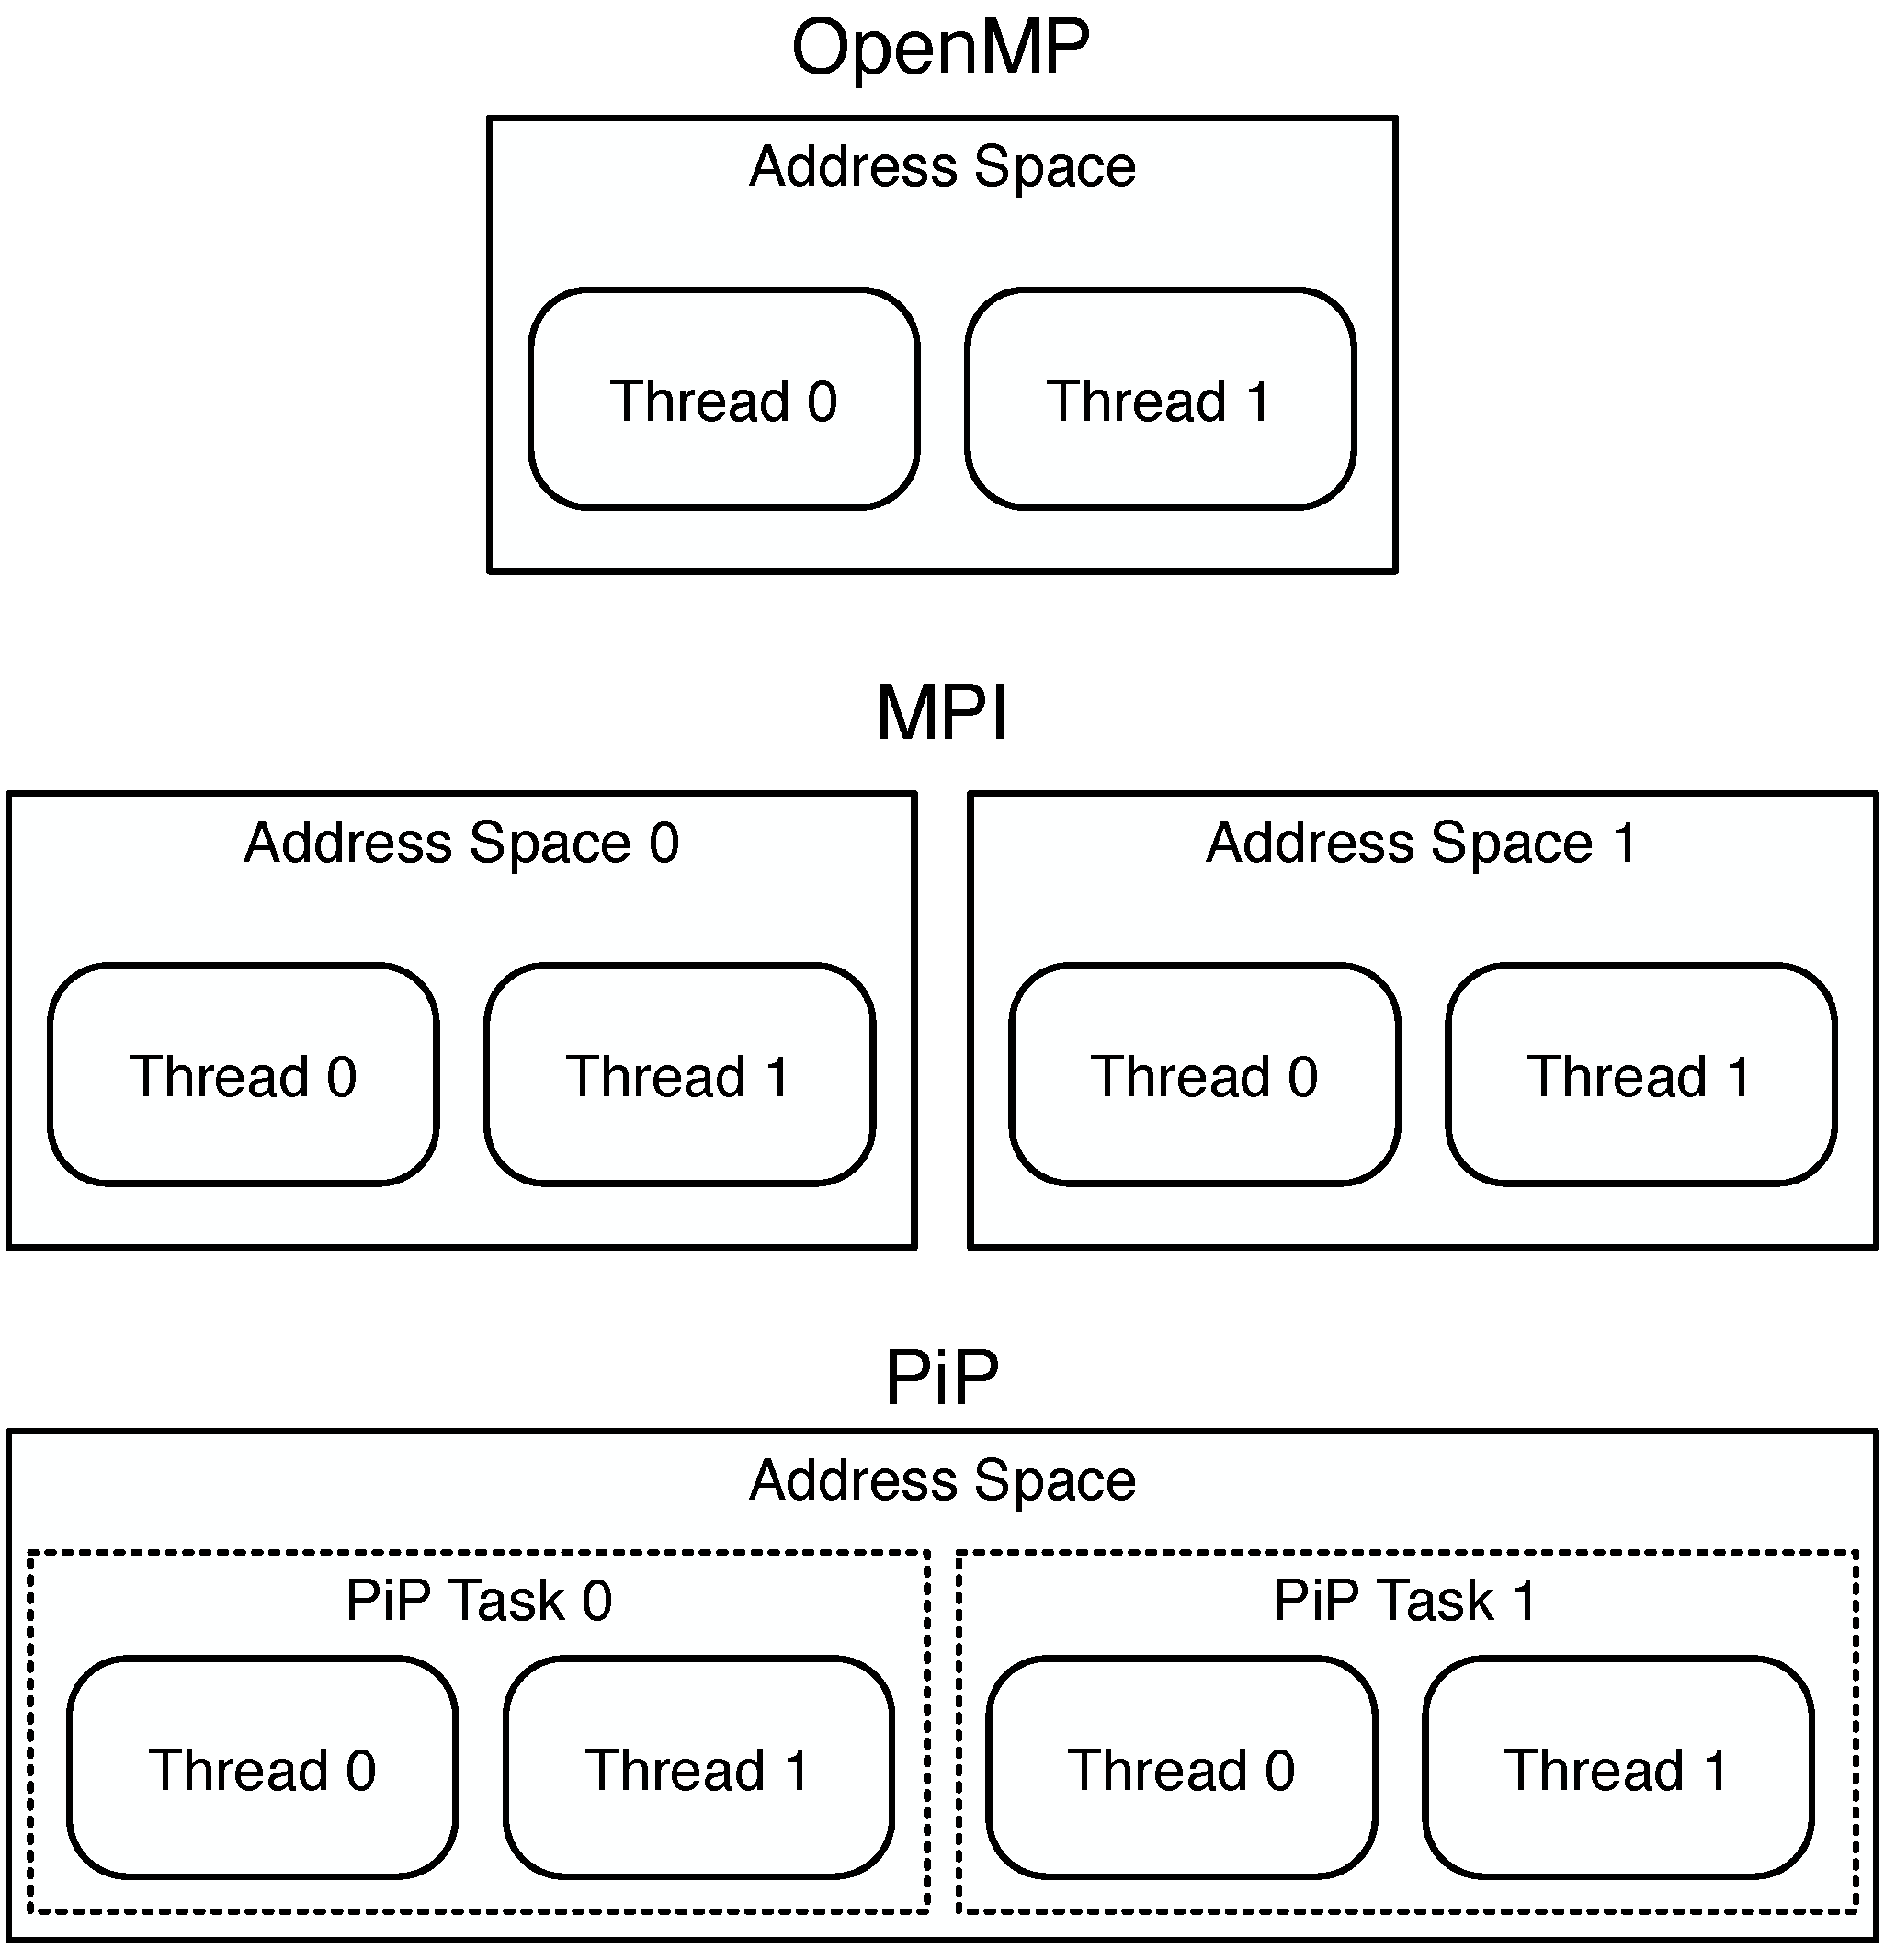
\includegraphics[width=0.7\columnwidth]{tasks/Figs/AddressSpace-OpenMP-MPI-PiP.pdf}
\caption{Differences of OpenMP, MPI and PiP}
\label{fig:tasks:hello-var-omp}
\end{figure}

Static variables are associated to an address space in the traditional
process model and thread model. Because of this, each process has its
own static variables, which are shared by all threads using the same
address space. Each PiP task is guaranteed to have its own static
variable set under the PiP execution model, decoupling from the
address space while maintaining address space sharing. {\it variable
  privatization} is what this is.

It is simple to share information among PiP tasks while maintaining
the independence of each PiP task's execution thanks to the nature of
PiP, which includes privatized variables and sharing an address
space. The ``Hello World'' program has so far been proved to be able to
execute as PiP tasks concurrently, although this program is quite
basic and there is no information exchange between PiP tasks. We'll
demonstrate how information can be shared between PiP processes in the
section after this one.

\subsection{Export and Import}

If the address of the information to be exchanged is known, sharing an
address space allows data owned by a PiP task to be accessed. The
address of the shared data can be broadcast by a PiP task, and the
other PiP task(s) can obtain the published address.  

To start, each PiP task has a {\PIPID} that helps it stand out from the
rest. By giving the {\PIPID} of the exporting PiP task, other PiP tasks
that share the same address space can import the exported address.

\lstinputlisting[style=program,
  caption={Export and Import ({\tt export-import})},
  label=prg:export-import] {tasks/examples/export-import.c}

In this program, after adjusting the value of {\tt argv[1]}, a PiP
task with a PIPID of zero (zero) exports the address of the variable
{\tt x} by using \pipfunc{pip_named_export}. By using the
\pipfunc{pip_named_import} function, the 
remaining PiP tasks import the address that PiP task 0 exported. An
outcome of this program's execution is shown below. The other PiP
tasks can view the value that PiP task 0 exported, as demonstrated.

\lstinputlisting[style=example, 
  caption={Execution of Export and Import},
  label=out:export-import] {tasks/examples/export-import.out}

The address with the specified name is published by the
\pipfunc{pip_named_export} function. The
\pipfunc{pip_named_import} function blocking-waits for the specified
PiP job by {\PIPID} to reach the defined address. To avoid a race condition,
it is not permitted to export an address with the same name more than
once for the purpose of updating the address.

The PiP library's functions almost always return an integer value as
an error code. A return code of zero (zero) denotes success. This
error code is identical to those that Linux defines. Due to simplicity
and clarity, the returned code is not tested in the examples presented
thus far and moving forward.  

It is forbidden in \term{MPI} to access the data that is held by other
processes running on the same node\footnote{Strictly speaking, some
  \term{MPI} implementations based on the thread model may allow
  this. Major \term{MPI} implementation, such MPICH, 
Open MPI, and many other \term{MPI} implementations provided by vendors are
based on the process model, and there is no way to access data owned by
the other \term{MPI process}.}. In MPI, communication is the sole 
permitted method. Communication fundamentally entails copying data in
some way (done by software or hardware). Data copying consumes memory,
power, and time.

